\documentclass[compress]{beamer}
\usepackage[utf8]{vntex}
\usepackage{longtable,booktabs}
\usepackage{amsmath}
\usepackage{amsfonts}
\usepackage{cases}
\usepackage{amssymb}
\usepackage[utf8]{inputenc}
\usepackage[absolute,overlay]{textpos}
\usepackage{listings}
\usepackage{subcaption}
\usepackage{tikz}
\usepackage{pgfplots}
\usepackage{fancybox}
\usepackage{multirow}
\usepackage{tikz-uml}
\tikzumlset{font=\tiny}
\usepackage{multimedia}
\usetikzlibrary{arrows.meta}
\usetikzlibrary{shapes.geometric}
\PassOptionsToPackage{hyphens}{url}\usepackage{hyperref}  
\lstset{
	language = Java,
	frame = single,
	tabsize = 3
}

\usetheme{Warsaw}
%\usetheme{Antibes}
%\usecolortheme{spruce}
%\setbeamercolor{structure}{fg=cyan!90!blue}
%\newtheorem{theorem}{Định lý}[]

\expandafter\def\expandafter\insertshorttitle\expandafter{%
    \insertshorttitle\hfill%
    \insertframenumber\,/\,\inserttotalframenumber}
      
\AtBeginSection[] % Do nothing for \section*
{
\begin{frame}
\tableofcontents[currentsection]
\end{frame}
}
\AtBeginSubsection[] % Do nothing for \section*
{
\begin{frame}
\tableofcontents[currentsection, currentsubsection]
\end{frame}
}

\title[Mật mã trên đường cong Elliptic Curves cho thiết bị IoT]{Mật mã trên đường cong Elliptic Curves cho thiết bị IoT} 

\author[Đặng Quang Trung]{
Sinh viên thực hiện\\
Đặng Quang Trung - 20134145 \\[1em]
Giảng viên hướng dẫn\\
TS Trần Vĩnh Đức}
\begin{document}

\begin{frame}[plain]
\titlepage
\end{frame}

\begin{frame}[plain]{Nội dung trình bày}
\tableofcontents
\end{frame}

\section{Cở sở lý thuyết}
\begin{frame}{Tại sao cần có mật mã?}
\begin{figure}[h]
\begin{subfigure}{.35\textwidth}
  \centering
  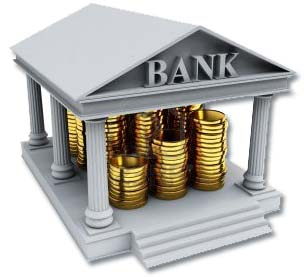
\includegraphics[width=1\linewidth]{../bank.jpg}
  %\caption{elliptic trên trường số thực}
  \label{fig:sfig1}
\end{subfigure}%
\begin{subfigure}{.35\textwidth}
  \centering
  
\includegraphics[width=1\linewidth]{../email.png}
  %\caption*{elliptic trên trường hữu hạn $\mathbb{F}_{29}$}
  \label{fig:sfig2}
\end{subfigure}
\end{figure}
\begin{figure}[h]
\begin{subfigure}{.35\textwidth}
  \centering
  
\includegraphics[width=1\linewidth]{../pay.png}
  %\caption*{elliptic trên trường hữu hạn $\mathbb{F}_{29}$}
  \label{fig:sfig2}
\end{subfigure}
\begin{subfigure}{.35\textwidth}
  \centering
  
\includegraphics[width=1\linewidth]{../soical.jpeg}
  %\caption*{elliptic trên trường hữu hạn $\mathbb{F}_{29}$}
  \label{fig:sfig2}
\end{subfigure}
%\caption{Đường cong elliptic dạng $y^2 = x^3 + 3x + 8$}
\label{fig:fig}
\end{figure}
\end{frame}
\begin{frame}{Ứng dụng}
\begin{itemize}
\item Thương mại điện tử:
\begin{itemize}
\item Chữ ký điện tử.
\item Mã hóa thông tin giao dịch.
\end{itemize}
\item Mạng xã hội:
\begin{itemize}
\item Mã hóa tin nhắn, văn bản,thư điện tử, \ldots .
\end{itemize}
\item Banking
\begin{itemize}
\item Xác thực người dùng
\item Mã hóa giao dịch, thông tin khách hàng.
\item \ldots.
\end{itemize}
\end{itemize}
\end{frame}
\subsection{Hệ mã khóa công khai}
\begin{frame}{Sơ đồ hệ mã khóa công khai}
\begin{center}
\begin{figure}[H]
\centering
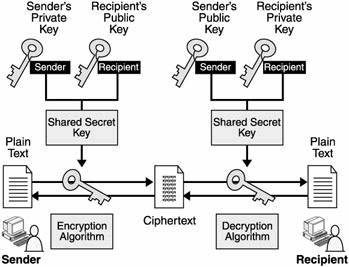
\includegraphics[width=0.65\linewidth]{../3.jpg}
\end{figure}
\end{center}
\end{frame}
\subsection{Giao thức Diffe-Hellman}
\begin{frame}{Diffe-Hellman}
\begin{center}
\begin{figure}
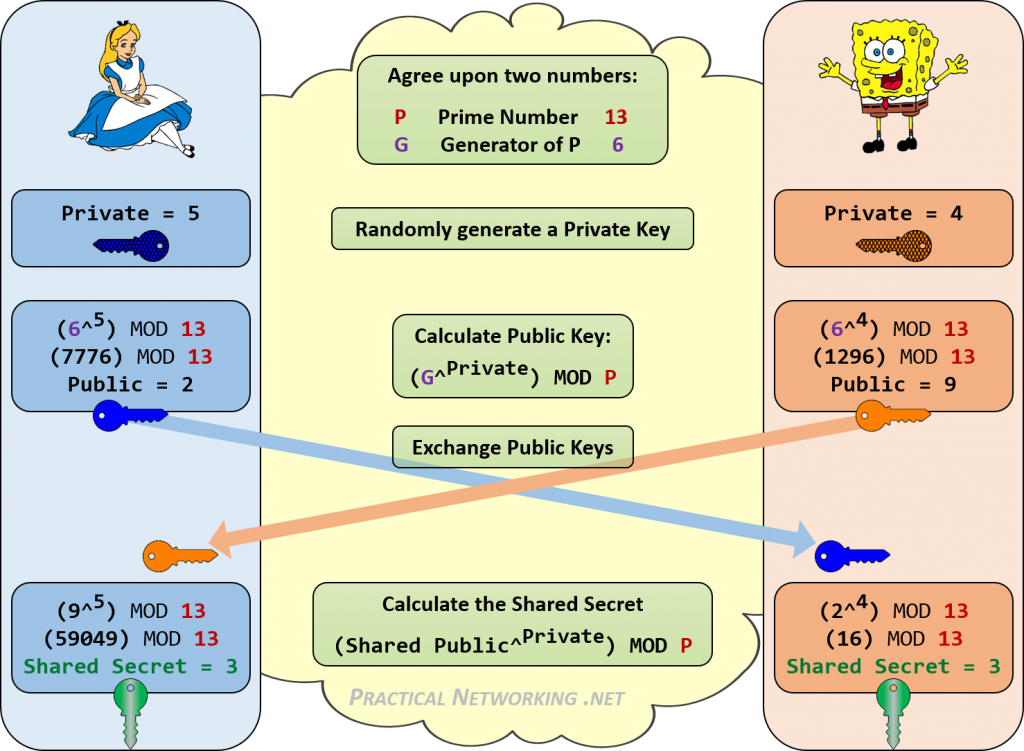
\includegraphics[width=0.9\linewidth]{../diffe-hellman.png}
\end{figure}
\end{center}
\end{frame}
\section{Đường cong elliptic}
\begin{frame}{Định nghĩa}
Một đường cong elliptic curve được xác định bởi phương trình đường cong
\begin{itemize}
\item \textbf{phương trình dạng Weierstrass}
\begin{displaymath}
E: y^2 = x^3 + Ax + B
\end{displaymath}
với điều kiện $A, B \in \mathbb{F}$ thỏa mãn $4A^3 + 27B^2 \neq 0$.
\item \textbf{phương trình dạng Montgomery}
\begin{displaymath}
M_{A,B}: By^2 = x^3 + Ax^2 + x 
\end{displaymath}
với điều kiện $A \in \mathbb{F} \setminus \{-2, 2\}, B 	\in \mathbb{F} \setminus \{0\}$ và $B(A^2 - 4) \neq 0$ 
\end{itemize}
\end{frame}
\begin{frame}{Elliptic trên trường hữu hạn}
\begin{figure}[h]
\begin{subfigure}{.5\textwidth}
  \centering
  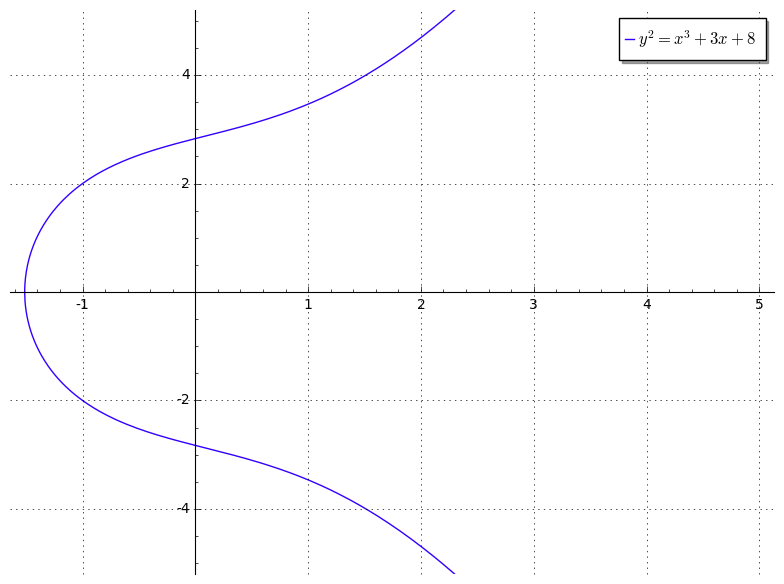
\includegraphics[width=1\linewidth]{../im11.png}
  \caption{elliptic trên trường số thực}
  \label{fig:sfig1}
\end{subfigure}%
\begin{subfigure}{.5\textwidth}
  \centering
  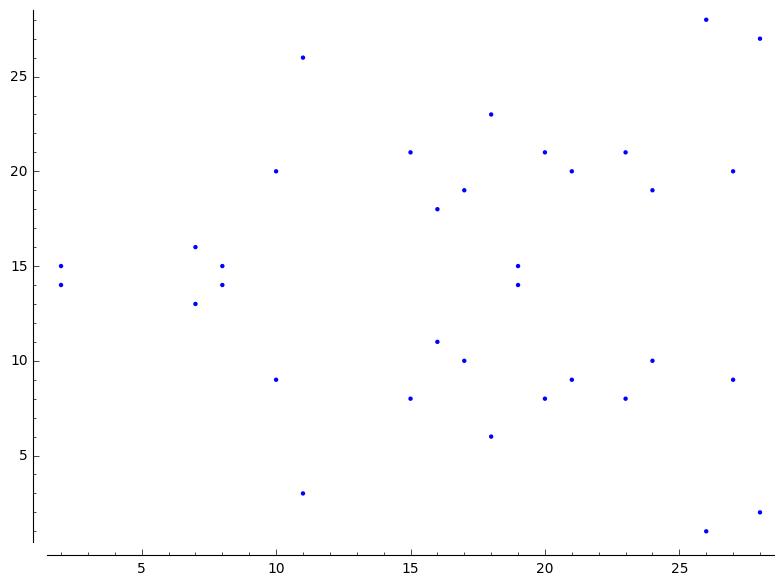
\includegraphics[width=1\linewidth]{../im12.png}
  \caption*{elliptic trên trường hữu hạn $\mathbb{F}_{29}$}
  \label{fig:sfig2}
\end{subfigure}
\caption{Đường cong elliptic dạng $y^2 = x^3 + 3x + 8$}
\label{fig:fig}
\end{figure}
\begin{itemize}
\item Đường cong elliptic có điểm giả định $\mathcal{O}$ ở vô cùng được gọi là điểm cơ sở.
\end{itemize}
\end{frame}
\begin{frame}{Luật trên đường cong elliptic hữu hạn}
Trên đường cong elliptic có 2 phép toán quan trọng là:
\begin{itemize}
\item Phép cộng (Add)
\item Phép nhân đôi và cộng (Double-And-Add)
\end{itemize}
Phép cộng 2 trên đường cong elliptic($E$) thoả mãn tính chất:
\begin{itemize}
\item Phần tử đơn vị: $P + \mathcal{O} = \mathcal{O} + P = P \ \forall P \in E$.
\item Phần tử nghịch: $P + (-P) = \mathcal{O} \ \forall P \in E$.
\item Kết hợp: $(P + Q) + R = P + (Q + R) \ \forall P,Q,R \in E$.
\item Giao hoán: $P + Q = Q + P \ \forall P,Q \in E$.
\end{itemize}
Hay nói cách khác tập các điểm thuộc $E$ với luật cộng tạo thành nhóm $Abelian$.
\end{frame}
\begin{frame}{Phép cộng trên đường cong elliptic}
\begin{figure}[h]
\begin{subfigure}{.5\textwidth}
  \centering
  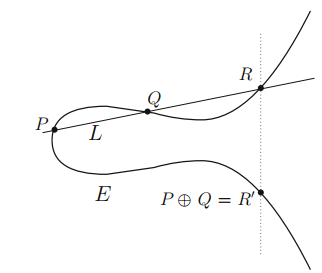
\includegraphics[width=0.85\linewidth]{../im2.png}
  \caption{$P + Q (P \neq Q)$}
  \label{fig:sfig1}
\end{subfigure}%
\begin{subfigure}{.5\textwidth}
  \centering
  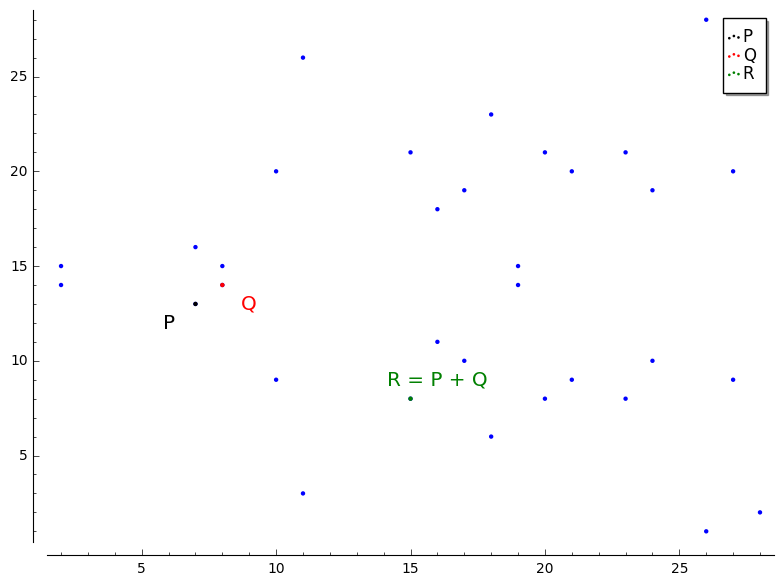
\includegraphics[width=1\linewidth]{../im13.png}
  \caption{$P + Q (P \neq Q)$ trên $\mathbb{F}_{29}$}
  \label{fig:sfig2}
\end{subfigure}
\caption*{Đường cong elliptic dạng $y^2 = x^3 + 3x + 8$}
\label{fig:fig}
\end{figure}
\begin{itemize}
\item \small{$P(7, 13) + Q(8, 14) = R(15, 8) \ (mod \ 29)\in E(\mathbb{F}_{29})$}.
\end{itemize}
\end{frame}
\begin{frame}{Phép cộng trên đường cong elliptic}
\begin{figure}[h]
\begin{subfigure}{.5\textwidth}
  \centering
  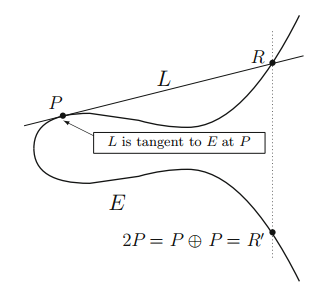
\includegraphics[width=0.85\linewidth]{../im3.png}
  \caption{$P + P ([2]P)$}
  \label{fig:sfig1}
\end{subfigure}%
\begin{subfigure}{.5\textwidth}
  \centering
  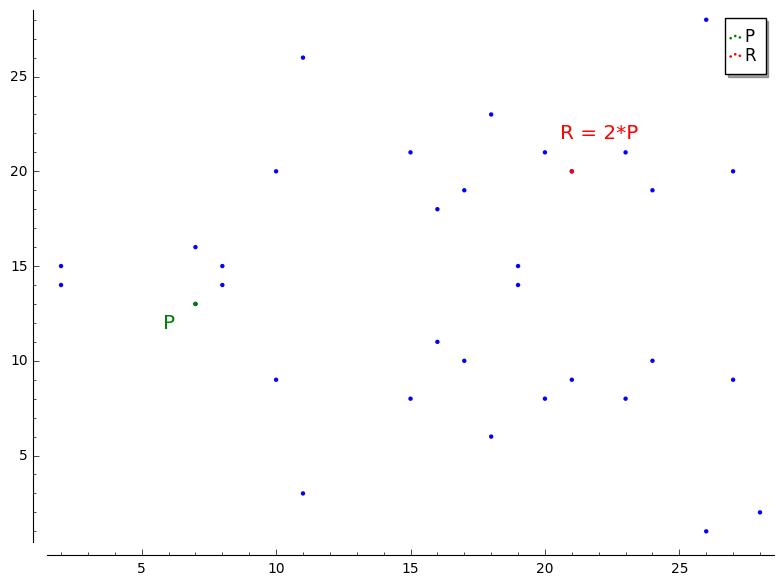
\includegraphics[width=1\linewidth]{../im14.png}
  \caption{$P + P ([2]P)$ trên $\mathbb{F}_{29}$}
  \label{fig:sfig2}
\end{subfigure}
\caption*{Đường cong elliptic dạng $y^2 = x^3 + 3x + 8$}
\label{fig:fig}
\end{figure}
\begin{itemize}
\item \small{$P(7 ,13) + P(7, 13) = 2P(7, 13) = R(21, 20) \ (mod 29) \in E(\mathbb{F}_{29})$}
\end{itemize}
\end{frame}
\begin{frame}{Phép cộng trên đường cong elliptic}
\begin{figure}[h]
\begin{subfigure}{.5\textwidth}
  \centering
  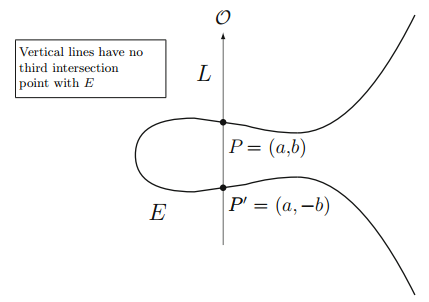
\includegraphics[width=1\linewidth]{../im4.png}
  \caption{$P + (-P)$}
  \label{fig:sfig1}
\end{subfigure}%
\begin{subfigure}{.5\textwidth}
  \centering
  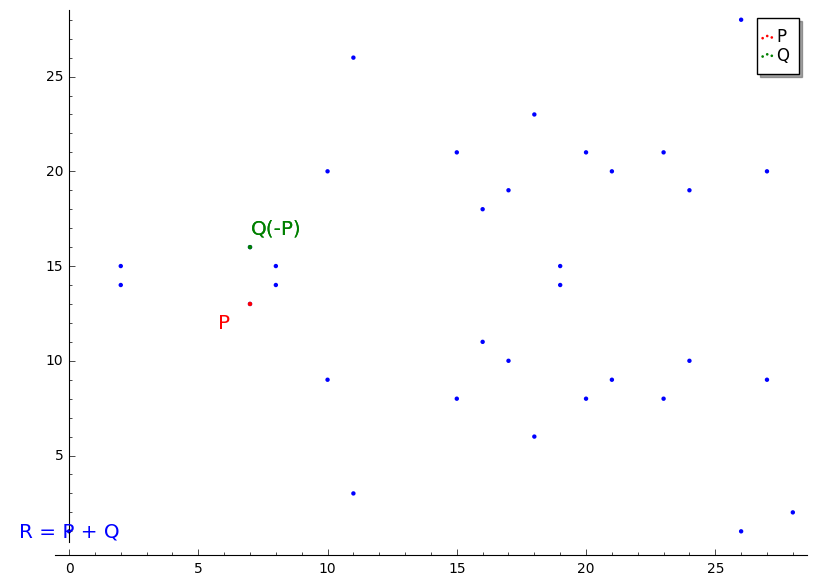
\includegraphics[width=1\linewidth]{../im15.png}
  \caption{$P + (-P)$ trên $\mathbb{F}_{29}$}
  \label{fig:sfig2}
\end{subfigure}
\caption*{Đường cong elliptic dạng $y^2 = x^3 + 3x + 8$}
\label{fig:fig}
\end{figure}
\begin{itemize}
\item \small{$P(7 ,13) + P'(7, 15) = \mathcal{O} \in E(\mathbb{F}_{29})$}
\begin{itemize}
\item \small{$-P(7, 13) = P'(7, -13) = P'(7, 15) \ (mod \ 29)$}
\end{itemize}
\item \small{$P + \mathcal{O} = P \ \forall P \in E(\mathbb{F}_{29})$}
\end{itemize}
\end{frame}
\begin{frame}{Double-And-Add}
Phép toán $Q = nP$ với $n \in \mathbb{F}_p$.
\begin{displaymath}
Q = \underbrace{P + P + \ldots + P}_{n \ add}
\end{displaymath}
Vấn đề:
\begin{itemize}
\item Nếu $n$ lớn thì tốc độc tính $Q = nP$ sẽ rất lâu.
\end{itemize}
Ta có thể biểu diễn $n$ thành:
\begin{displaymath}
n = n_0 + n_1 \cdot 2 + n_2 \cdot 4 + n_3 \cdot 8 + \ldots + n_r \cdot 2^r 
\end{displaymath}
với $n_0, n_1, \ldots, n_r \in \{0,1\}$. Nếu $n_r = 1$ ta có thể tính:
\begin{displaymath}
Q_0 = P, Q_1 = 2Q_0, Q_2 = 2Q_1, \ldots, Q_r = 2Q_{r-1}
\end{displaymath}
Chú ý rằng $Q_i$ chỉ gấp 2 lần $Q_{i - 1}$ hay $Q_i = 2^iP$.Phép cộng sẽ được tính:
\begin{displaymath}
nP = n_0Q_0 + n_1Q_1 + n_2Q_2 + \ldots + n_rQ_r
\end{displaymath}
\end{frame}
\begin{frame}{Điểm sinh trên đường cong}
Cho $G$ là một điểm nằm trên $E$ và có cấp là $n$ (hay $nG = \mathcal{O}$). Khi đó các phần tử của đường cong sẽ biễu diễn bởi:
\begin{displaymath}
G, 2G, 3G, 4G, \ldots, nG
\end{displaymath}
với $nG = \mathcal{O}$ là điểm cơ sở.
\end{frame}
\begin{frame}{Ví dụ}
Cho pt $y^2 = x^3 + 3x + 8$, ta có điểm sinh $G = (19, 15)$ có cấp $n = 35$
\small{
\begin{center}
\begin{tabular}{lllllllll}
$G = (19, 15)$ & & $2G = (15, 8)$ & & $3G = (18, 23)$ & & $4G = (27, 20)$ \\
$5G = (21, 20)$ & & $6G = (17, 19)$ & & $7G = (26, 28)$ & & $8G = (20, 8)$ \\
$9G = (10, 9)$ & & $10G = (23, 21)$ & & $11G = (11, 26)$ & & $12G = (24, 10)$ \\
$13G = (16, 11)$ & & $14G = (28, 2)$ & & $15G = (7, 16)$ & & $16G = (2, 15)$ \\
$17G = (8, 14)$ & & $18G = (8, 15)$ & & $19G = (2, 14)$ & & $20G = (7, 13)$ \\
$21G = (28, 17)$ & & $22G = (16, 18)$ & & $23G = (24, 19)$ & & $24G = (11, 3)$ \\
$25G = (23, 8)$ & & $26G = (10, 20)$ & & $27G = (20, 21)$ & & $28G = (26, 1)$ \\
$29G = (17, 10)$ & & $30G = (21, 9)$ & & $31G = (27, 9)$ & & $32G = (18, 6)$ \\
$33G = (15, 21)$ & & $34G = (19, 14)$ & &$35G = \mathcal{O}$ \\
\end{tabular}
\end{center}
}
\end{frame}
\begin{frame}{Diffe-Hellman trên đường cong Elliptic}
\begin{flushleft}
\footnotesize{
\begin{tabular}{lcl}
      &  Cả Alice và Bob cùng thống nhất thông số &   \\
Alice &  số nguyên tố p, đường cong E trên trường $\mathbb{F}_p$ & Bob \\
      &  và điểm sinh G                                          &  \\
\hline \\
      &   $p = 29, E: y^2 = x^3 + 3x + 8$ trên $\mathbb{F}_{29}$ &  \\
      &  và điểm sinh $G = (19, 15)$ & \\
\hline \\ 
$n_A = 7$ &  Alice gửi $Q_A$ cho Bob $\overrightarrow{ \ \ \ \ \ \ \ \ \ \  \ \ \ } Q_A$    &$n_B = 8$  \\
$Q_A = n_A\cdot G$ & $Q_B \overleftarrow{ \ \ \ \ \ \ \ \ \ \  \ \ \ }$ Bob gửi $Q_B$ cho Alice                        &$Q_B = n_B\cdot G$ \\
$\ \ \ \ \ = (26, 28) $ &                           &$\ \ \ \ \ = (20, 8)$ \\
\hline \\
      & Tính khóa chia sẻ giữa Alice và Bob & \\
\hline \\
$S = n_A\cdot Q_B$ &  $S = (n_A\cdot n_B)\cdot G = (n_B\cdot n_A)\cdot G$ & $S = n_B\cdot Q_A$ \\
$\ \ \ = (28, 27)$ &                    &$\ \ \ = (28, 27)$
\end{tabular}
}
\end{flushleft}
\end{frame}
\section{Chứng thư số ẩn}
\begin{frame}{Tại sao cần chứng thư số ẩn?}
\begin{center}
\begin{figure}
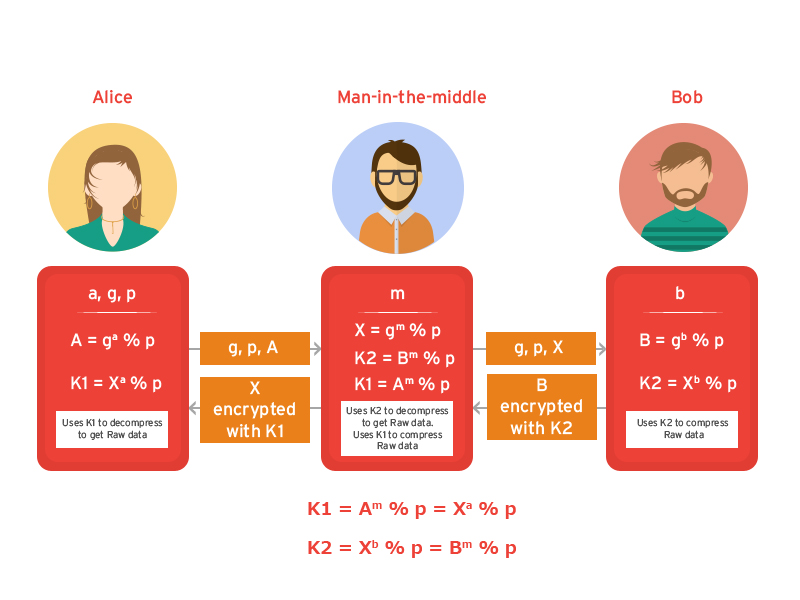
\includegraphics[width=0.8\linewidth]{../amit.jpg}
\caption*{Tấn công MITM}
\end{figure}
\end{center}
\end{frame}
\begin{frame}{Sơ đồ PKI}
\begin{center}
\begin{figure}
\centering
\includegraphics[width=0.8\linewidth]{../PKI.png}
\caption*{Sơ đồ PKI}
\end{figure}
\end{center}
\end{frame}
\begin{frame}{Chứng thư số ẩn ECQV}
Sơ đồ chứng thư số ẩn bao gồm các phần:
\small{
\begin{itemize}
\item[1. ] \textbf{ECQV\_Setup}: CA thiết lập các tham số đường cong elliptic, hàm băm, định dạng mã hóa chứng chỉ và tất cả các bên đã chọn một trình tạo số ngẫu nhiên. CA tạo ra một cặp khóa.
\item[2. ] \textbf{Cert\_Request}: Người yêu cầu U phải tạo một yêu cầu cho một chứng chỉ, được gửi đến CA.
\item[3. ] \textbf{Cert\_Generate}: Khi nhận được yêu cầu chứng chỉ từ U, CA xác nhận danh tính của U và tạo chứng chỉ số ẩn. CA gửi phản hồi cho U.
\item[4. ] \textbf{Cert\_PK\_Extraction}: Với chứng chỉ số ẩn cho U người dùng, thông số và khóa công khai của CA.
\item[5. ] \textbf{Cert\_Reception}: Sau khi nhận được phản hồi cho yêu cầu chứng chỉ của mình, U đảm bảo tính hợp lệ của cặp khóa được chứng nhận ngầm.
\end{itemize}
}
\end{frame}
\begin{frame}{Sơ đồ ECQV}
\begin{center}
\begin{figure}[h]
\centering
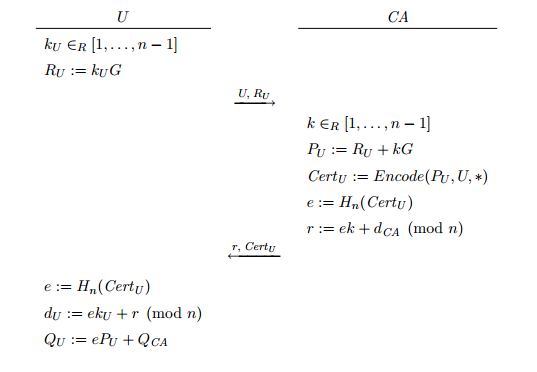
\includegraphics[width=0.85\linewidth]{../im8.png}
\end{figure}
\end{center}
\end{frame}
\section{Kết quả}
\section*{Cài đặt}
\begin{frame}{Cài đặt}

\end{frame}
\section*{Kết quả thu được}
\begin{frame}{Kết quả thu được}
\begin{itemize}
\item Tìm hiểu được một số nguyên lý mã công khai, hàm băm, chữ ký điện tử.
\item Hiểu được lý thuyết về đường cong elliptic.
\item Hiểu được các bước cơ bản xây dựng một đường cong elliptic và ứng dụng trong thuật toán trao đổi khóa và tạo chứng thư số.
\item Nắm được một số kiểu tấn công như timing-attack, tấn công xen giữa.
\item \ldots
\end{itemize}
\end{frame}
\section*{Hạn chế}
\begin{frame}{Hạn chế}
\begin{itemize}
\item Chưa tìm hiểu được một cách đầy đủ và chi tiết về đường cong elliptic trên trường hữu hạn $F_{2^m}$ với 2 dạng cơ sở normal và polinomial.
\item Ứng dụng truyền file và chứng thư số chưa có giao diện đẹp mắt và mới chỉ thử nghiệm trên một máy.
\item \ldots
\end{itemize}
\end{frame}
\section*{Hướng phát triển}
\begin{frame}{Hướng Phát triển}
\begin{figure}[h]
\begin{subfigure}{.3\textwidth}
  \centering
  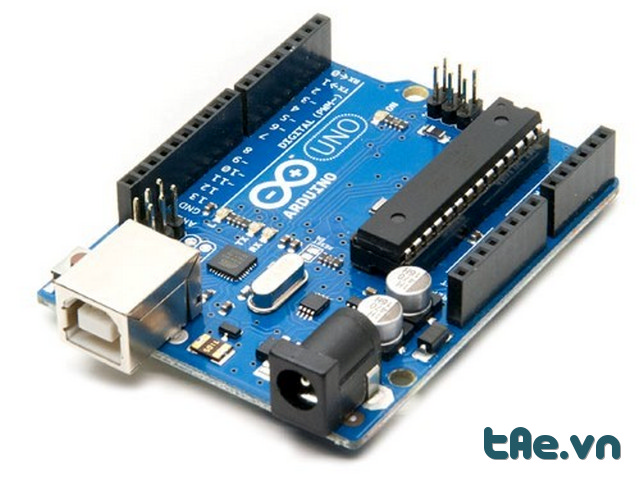
\includegraphics[width=1\linewidth]{../uno.jpg}
  %	\caption{1a elliptic trên trường số thực}
  \label{fig:sfig1}
\end{subfigure}%
\begin{subfigure}{.3\textwidth}
  \centering
  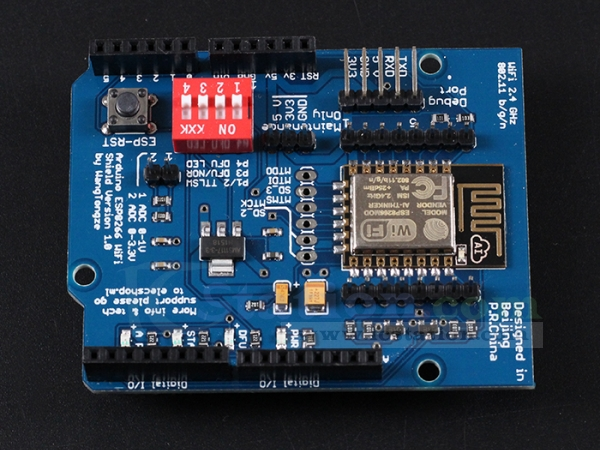
\includegraphics[width=1\linewidth]{../esp.jpg}
 % \caption{1b elliptic trên trường hưu hạn $\mathbb{F}_{29}$}
  \label{fig:sfig2}
\end{subfigure}
\begin{subfigure}{.3\textwidth}
  \centering
  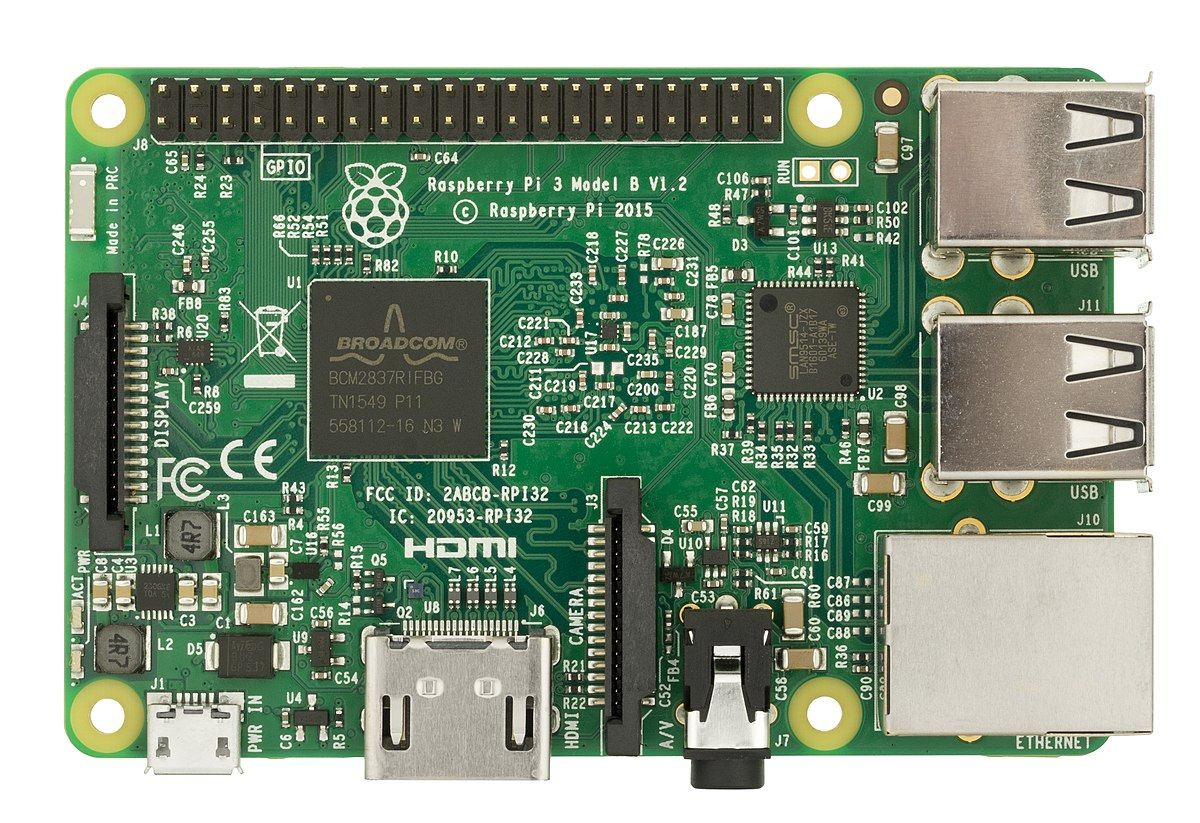
\includegraphics[width=1\linewidth]{../ras.jpg}
  \label{fig:sfig2}
\end{subfigure}
\caption{arduino, esp-12(esp8266), raspberry pi – các thiết bị dùng trong phát triển sản phẩm IoT} \label{h6.3}
\end{figure}
\begin{itemize}
\item Tốc độ tính toán trên đường cong Elliptic nhanh.
\item Lưu trữ và trao đổi khóa nhỏ gọn.
\item Tính an toàn bảo mật cao.
\end{itemize}
\end{frame}
\begin{frame}
\begin{center}
\begin{figure}
\centering

\includegraphics[width=1\linewidth]{../thanks.jpg}
\end{figure}
\end{center}
\end{frame}
\end{document}